\documentclass{article}

\usepackage[english]{babel}
\usepackage[utf8]{inputenc}
\usepackage{amsmath,amssymb}
\usepackage{parskip}
\usepackage{graphicx}
\usepackage{listings}
\usepackage{subfig}
\usepackage{float}
\lstset{
    numbers=left, 
    numberstyle= \tiny, 
    keywordstyle= \color{ blue!70},
    commentstyle= \color{red!50!green!50!blue!50}, 
    frame=shadowbox, % 阴影效果
    rulesepcolor= \color{ red!20!green!20!blue!20} ,
    escapeinside=``, % 英文分号中可写入中文
    xleftmargin=2em,xrightmargin=2em, aboveskip=1em,
    framexleftmargin=2em,
    breaklines=true,
    language=R
} 

% Margins
\usepackage[top=2.5cm, left=3cm, right=3cm, bottom=4.0cm]{geometry}
% Colour table cells
\usepackage[table]{xcolor}

% Get larger line spacing in table
\newcommand{\tablespace}{\\[1.25mm]}
\newcommand\Tstrut{\rule{0pt}{2.6ex}}         % = `top' strut
\newcommand\tstrut{\rule{0pt}{2.0ex}}         % = `top' strut
\newcommand\Bstrut{\rule[-0.9ex]{0pt}{0pt}}   % = `bottom' strut

%%%%%%%%%%%%%%%%%
%     Title     %
%%%%%%%%%%%%%%%%%
\title{CSCI946 Assignment}
\author{Yao Xiao \\ SID 2019180015}
\date{\today}

\begin{document}
\maketitle

%%%%%%%%%%%%%%%%%
%   Problem 1   %
%%%%%%%%%%%%%%%%%
\section{Task 1}
\begin{lstlisting}
library("ggplot2")
library("reshape2")
library("lda")

data(cora.documents)
data(cora.vocab)

theme_set(theme_bw())

K <- 10

N <- 9

result <- lda.collapsed.gibbs.sampler(cora.documents,
                                      K,
                                      cora.vocab,
                                      25,
                                      0.1,
                                      0.1,
                                      compute.log.likelihood=TRUE)


top.words <- top.topic.words(result$topics, 5, by.score=TRUE)

topic.props <- t(result$document_sums) / colSums(result$document_sums)

document.samples <- sample(1:dim(topic.props)[1], N)

topic.props <- topic.props[document.samples,]

topic.props[is.na(topic.props)] <- 1 / K

colnames(topic.props) <- apply(top.words, 2, paste, collapse=" ")

topic.props.df <- melt(cbind(data.frame(topic.props),document=factor(1:N)), variable.name="topic",id.vars = "document")

qplot(topic, value*100, fill=topic, stat="identity", ylab="proportion (%)", data=topic.props.df, geom="col") +
  theme(axis.text.x = element_text(angle=0, hjust=1, size=12)) + coord_flip() +
  facet_wrap(~ document, ncol=3)
\end{lstlisting}

\begin{figure}[H]
    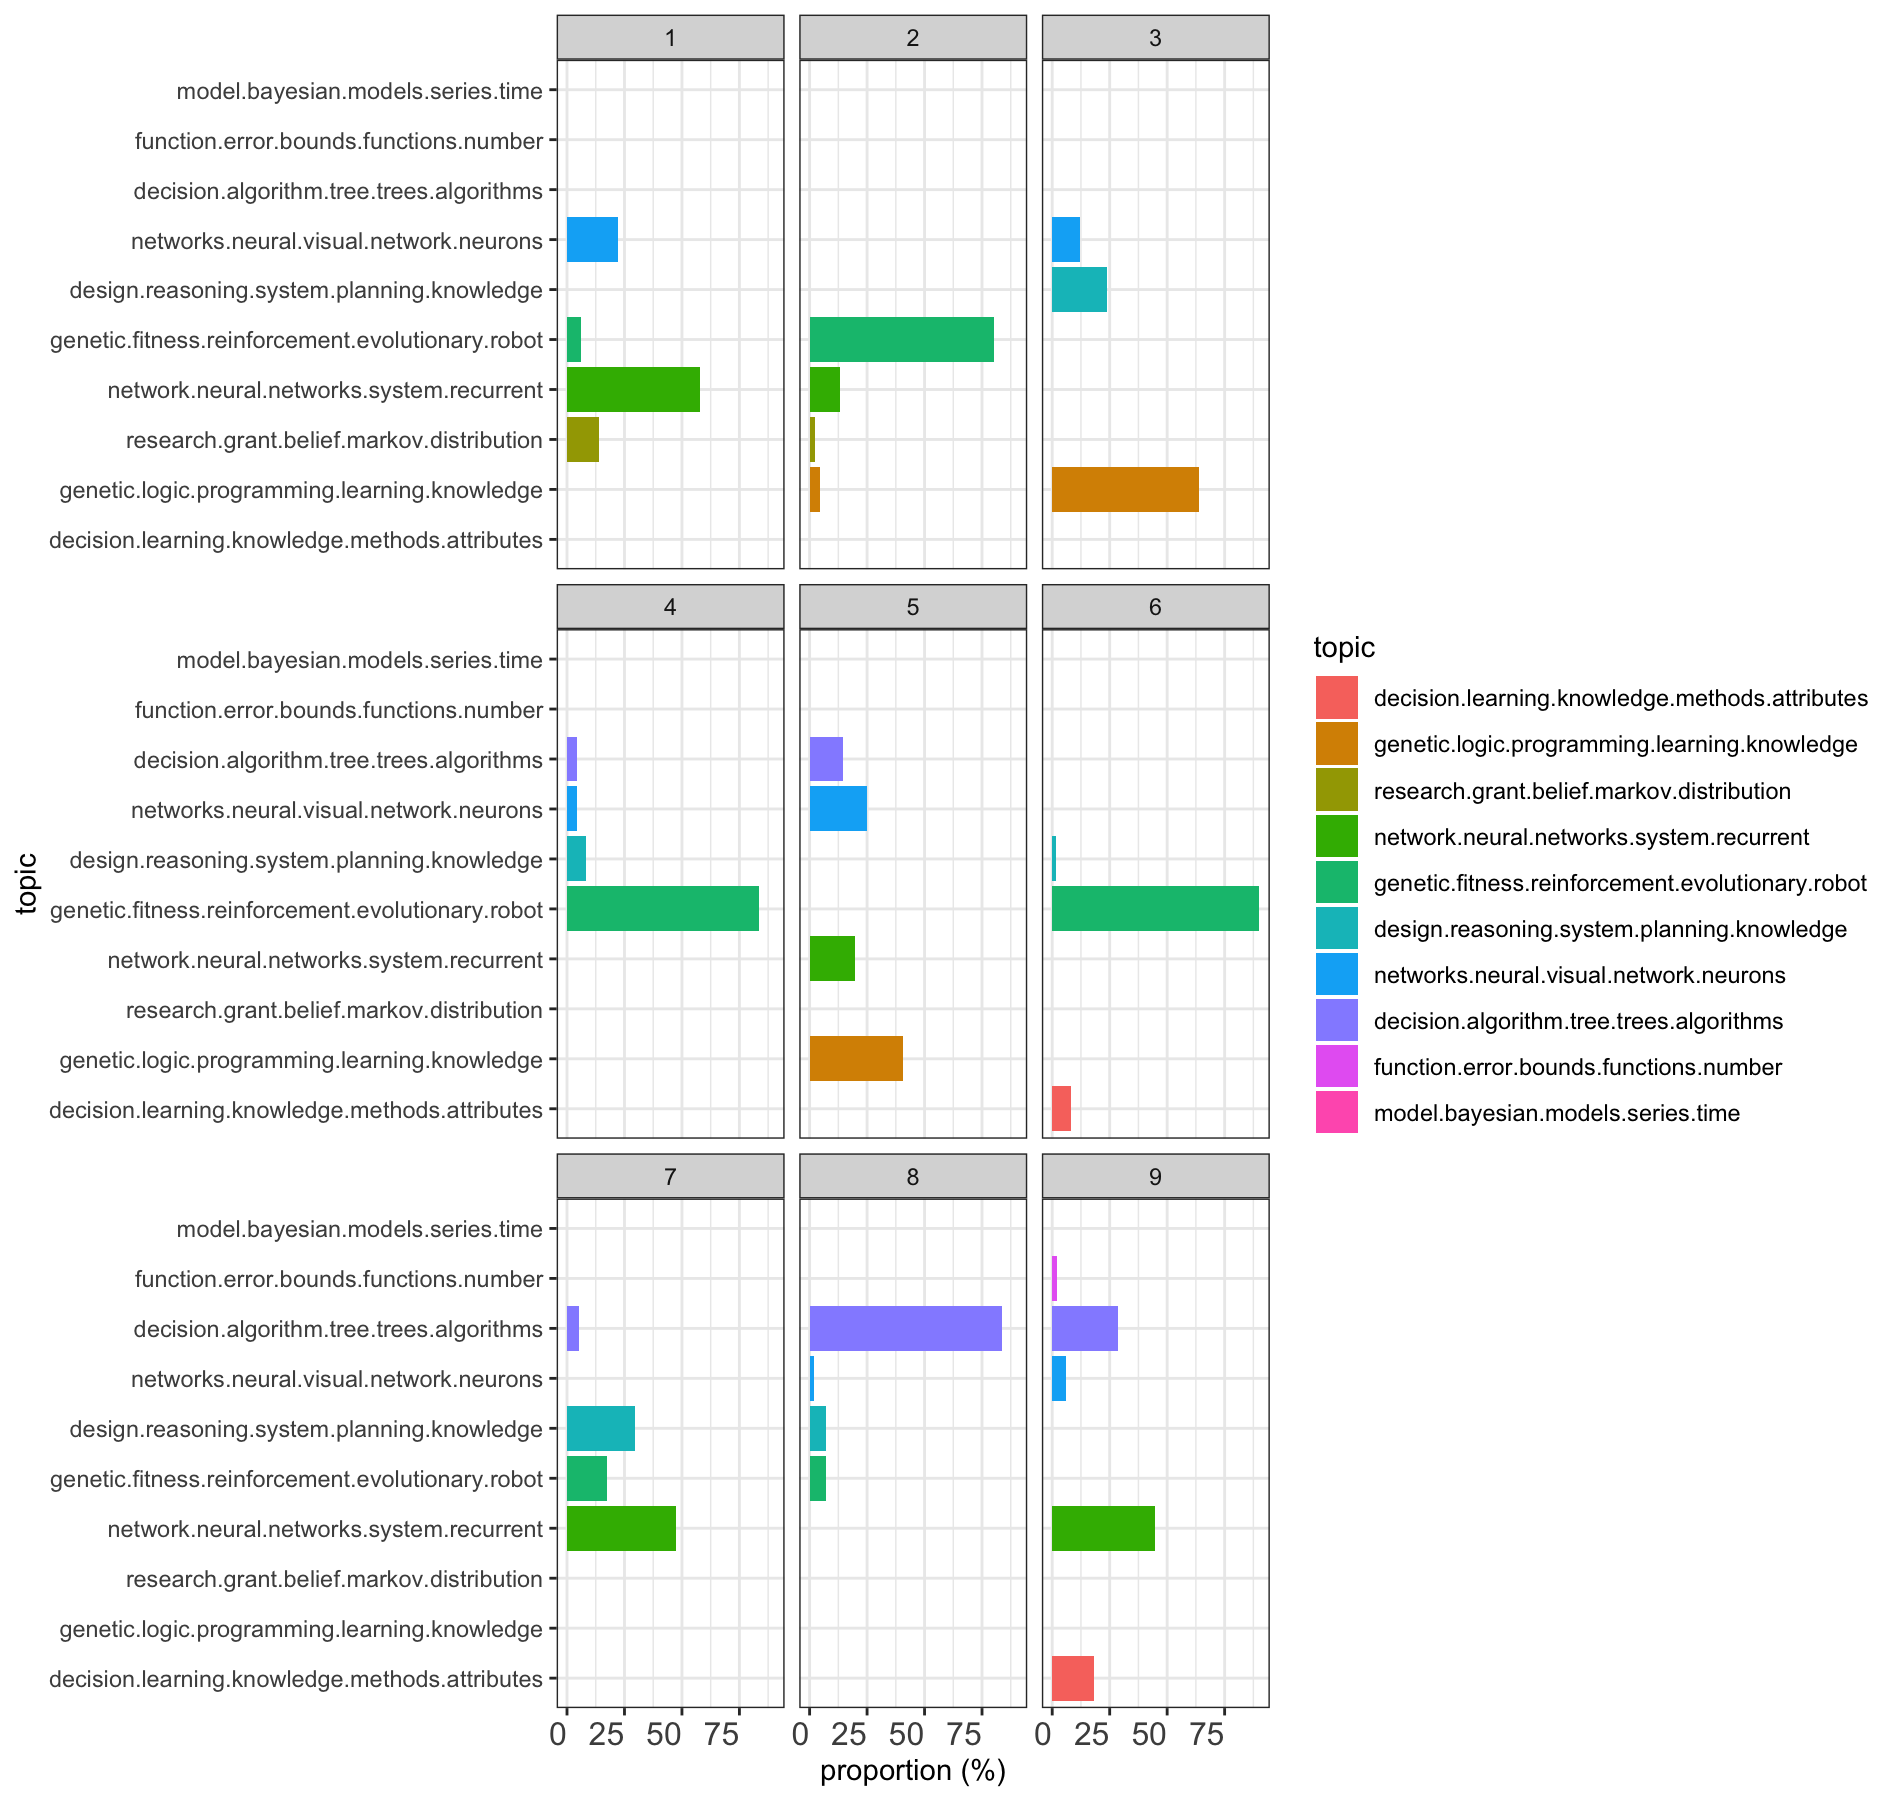
\includegraphics[width=1\textwidth]{Fig4}
\end{figure}

\section{Task 2}
\begin{lstlisting}
library("dplyr")
library("magrittr")
library("data.table")
library("tidytext")
library("topicmodels")
library("colorspace")
library("purrr")
library("ldatuning")
library("gmp")
library("RColorBrewer")
library("wordcloud")
library("ggplot2")
library("lubridate")
library("lubridate")
library("reshape2")
library("textmineR")

data <- fread("/Users/december/Desktop/Week8/Sentiment.csv")

data <- data %>% select(text,id) %>% head(5000)

# text cleaning
data$text <- sub("RT.*:", "", data$text)
data$text <- sub("@.* ", "", data$text)
text_cleaning_tokens <- data %>% 
  tidytext::unnest_tokens(word, text)
text_cleaning_tokens$word <- gsub('[[:digit:]]+', '', text_cleaning_tokens$word)
text_cleaning_tokens$word <- gsub('[[:punct:]]+', '', text_cleaning_tokens$word)
text_cleaning_tokens <- text_cleaning_tokens %>% filter(!(nchar(word) == 1))%>% 
  anti_join(stop_words)
tokens <- text_cleaning_tokens %>% filter(!(word==""))


tokens <- tokens %>% mutate(ind = row_number())
tokens <- tokens %>% group_by(id) %>% mutate(ind = row_number()) %>%
  tidyr::spread(key = ind, value = word)
tokens [is.na(tokens)] <- ""
tokens <- tidyr::unite(tokens, text,-id,sep =" " )
tokens$text <- trimws(tokens$text)

#create DTM
dtm <- CreateDtm(tokens$text, 
                 doc_names = tokens$id, 
                 ngram_window = c(1, 2))


# explore the basic frequency
tf <- TermDocFreq(dtm = dtm)
original_tf <- tf %>% select(term, term_freq,doc_freq)
rownames(original_tf) <- 1:nrow(original_tf)

# eliminate words appearing less than 2 times or in more than half of the doc
vocabulary <- tf$term[ tf$term_freq > 1 & tf$doc_freq < nrow(dtm) / 2 ]

dtm = dtm

# run LDA 
k_list <- seq(1, 20, by = 1)
model_dir <- paste0("models_", digest::digest(vocabulary, algo = "sha1"))
if (!dir.exists(model_dir)) dir.create(model_dir)
model_list <- TmParallelApply(X = k_list, FUN = function(k){
  filename = file.path(model_dir, paste0(k, "_topics.rda"))
  
  if (!file.exists(filename)) {
    m <- FitLdaModel(dtm = dtm, k = k, iterations = 500)
    m$k <- k
    m$coherence <- CalcProbCoherence(phi = m$phi, dtm = dtm, M = 5)
    save(m, file = filename)
  } else {
    load(filename)
  }
  
  m
}, export=c("dtm", "model_dir"))

# model tuning
# choosing the best model
coherence_mat <- data.frame(k = sapply(model_list, function(x) nrow(x$phi)), 
                            coherence = sapply(model_list, function(x) mean(x$coherence)), 
                            stringsAsFactors = FALSE)
ggplot(coherence_mat, aes(x = k, y = coherence)) +
  geom_point() +
  geom_line(group = 1)+
  ggtitle("Best Topic by Coherence Score") + theme_minimal() +
  scale_x_continuous(breaks = seq(1,20,1)) + ylab("Coherence")

# select models based on max average
model <- model_list[which.max(coherence_mat$coherence)][[ 1 ]]

# top 20 terms based on phi  
model$top_terms <- GetTopTerms(phi = model$phi, M = 20)
top20_wide <- as.data.frame(model$top_terms)

# word, topic relationship
# looking at the terms allocated to the topic and their pr(word|topic)
allterms <-data.frame(t(model$phi))
allterms$word <- rownames(allterms)
rownames(allterms) <- 1:nrow(allterms)
allterms <- melt(allterms,idvars = "word") 
allterms <- allterms %>% rename(topic = variable)
FINAL_allterms <- allterms %>% group_by(topic) %>% arrange(desc(value))


# topic,word,freq 
final_summary_words <- data.frame(top_terms = t(model$top_terms))
final_summary_words$topic <- rownames(final_summary_words)
rownames(final_summary_words) <- 1:nrow(final_summary_words)
final_summary_words <- final_summary_words %>% melt(id.vars = c("topic"))
final_summary_words <- final_summary_words %>% rename(word = value) %>% select(-variable)
final_summary_words <- left_join(final_summary_words,allterms)
final_summary_words <- final_summary_words %>% group_by(topic,word) %>%
  arrange(desc(value))
final_summary_words <- final_summary_words %>% group_by(topic, word) %>% filter(row_number() == 1) %>% 
  ungroup() %>% tidyr::separate(topic, into =c("t","topic")) %>% select(-t)
word_topic_freq <- left_join(final_summary_words, original_tf, by = c("word" = "term"))

# per-document-per-topic probabilities 
theta_df <- data.frame(model$theta)
theta_df$document <-rownames(theta_df) 
rownames(theta_df) <- 1:nrow(theta_df)
theta_df$document <- as.numeric(theta_df$document)
theta_df <- melt(theta_df,id.vars = "document")
theta_df <- theta_df %>% rename(topic = variable) 
theta_df <- theta_df %>% tidyr::separate(topic, into =c("t","topic")) %>% select(-t)
FINAL_document_topic <- theta_df %>% group_by(document) %>% 
  arrange(desc(value)) %>% filter(row_number() ==1)

# visualising of topics in a dendrogram 
model$topic_linguistic_dist <- CalcHellingerDist(model$phi)
model$hclust <- hclust(as.dist(model$topic_linguistic_dist), "ward.D")
model$hclust$labels <- paste(model$hclust$labels, model$labels[ , 1])
plot(model$hclust)


# visualising topics of words based on the max value
set.seed(1234)
pdf("result.pdf")
for(i in 1:length(unique(final_summary_words$topic)))
{  wordcloud(words = subset(final_summary_words ,topic == i)$word, freq = subset(final_summary_words ,topic == i)$value, min.freq = 1,
             max.words=200, random.order=FALSE, rot.per=0.35, 
             colors=brewer.pal(8, "Dark2"))}

dev.off()
\end{lstlisting}

\begin{figure}[H]
    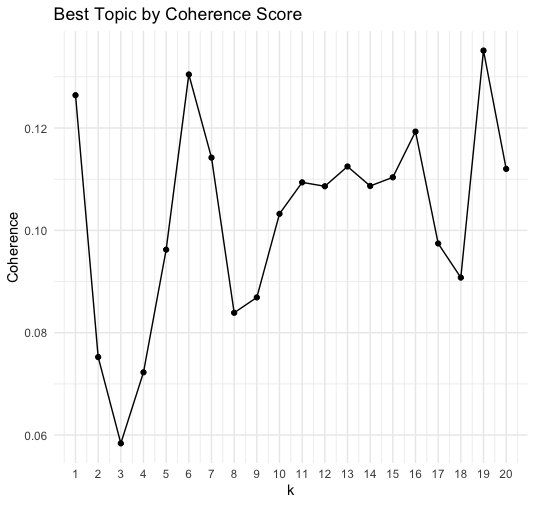
\includegraphics[width=0.95\textwidth]{Fig1}
\end{figure}

\begin{figure}[H]
    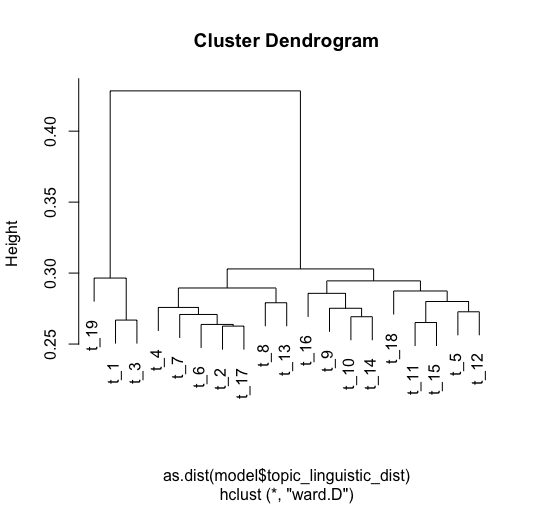
\includegraphics[width=0.95\textwidth]{Fig2}
\end{figure}

\begin{figure}
    \centering
    \caption{Word cloud of topic 3}
    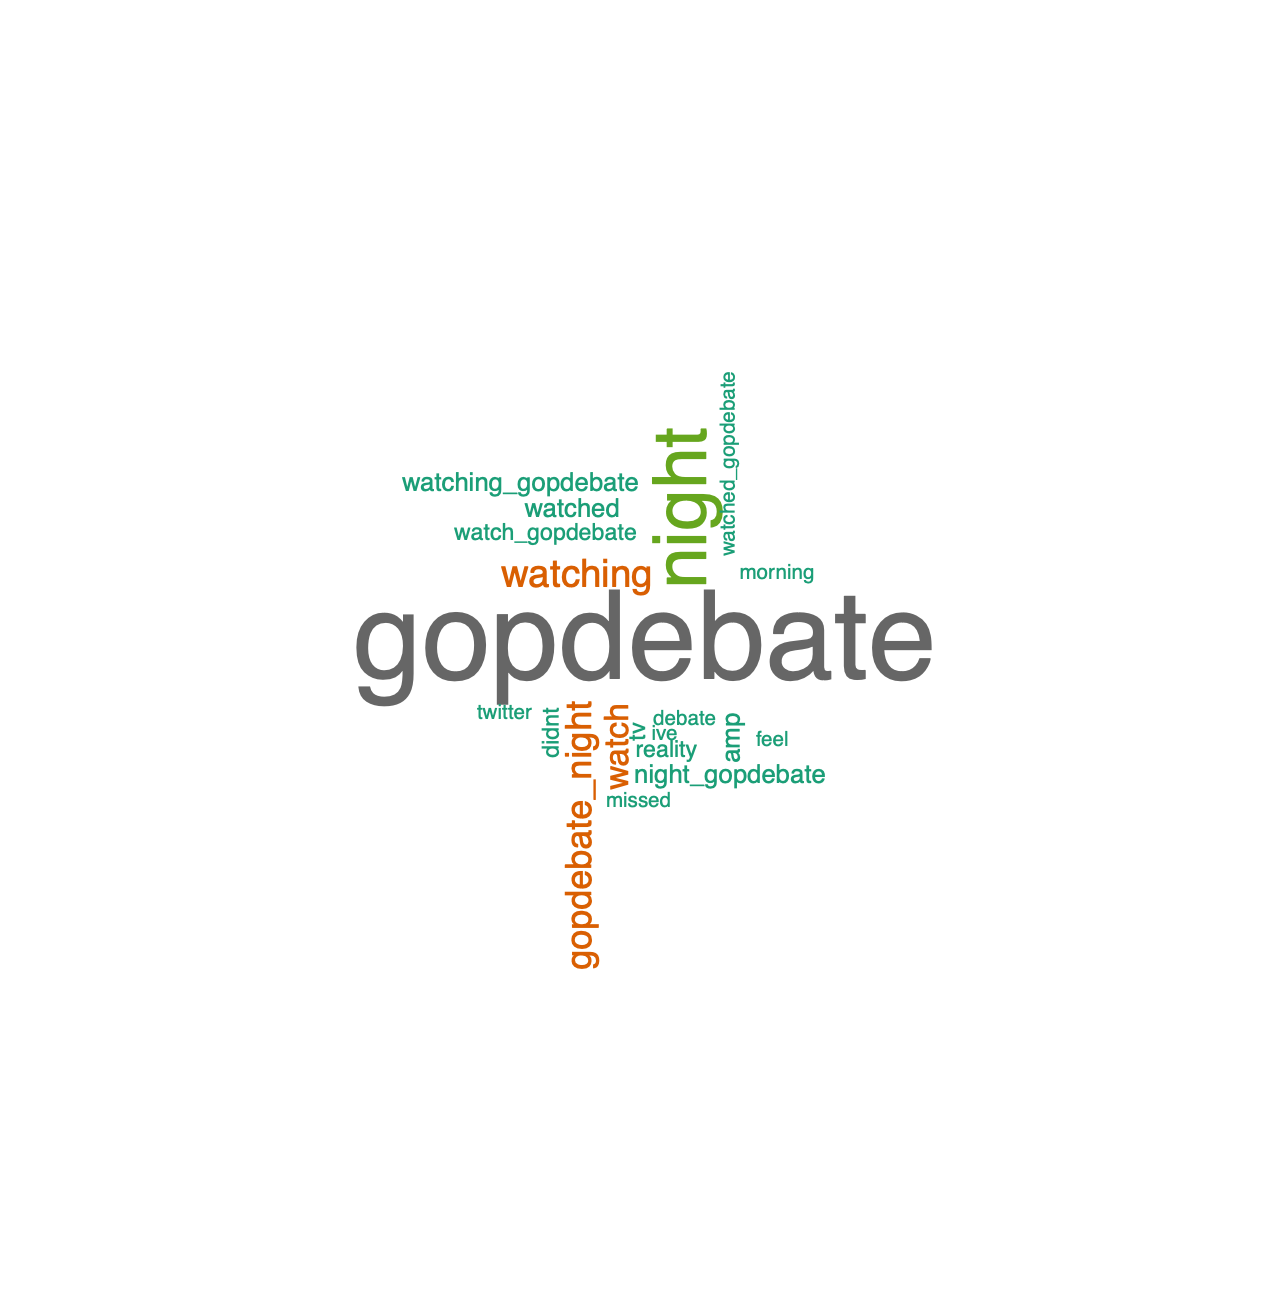
\includegraphics[width=1\textwidth]{Fig3}
\end{figure}


\end{document}
